\documentclass[twoside, 11pt]{article}

\usepackage{meta/ipcb}

\begin{document}

\thispagestyle{empty}
\noindent\hspace*{-1.5cm}
\includegraphics[width=6.4cm]{est}


\vspace*{90pt}

\title{ECSMoS: An ECS-based Pedestrian Mobility Simulator}

% \subtitle{ECS based pedestrian mobility simulatior}

\vspace*{36pt}

\cambria

\info{Rafael Souza Cotrim}

\vspace*{24pt}

\noindent\textbf{\large{Orientadores}}

\info{Alexandre José Pereira Duro da Fonte}

\info{João Manuel Leitão Pires Caldeira}

\vfill

\notice{Dissertação apresentada à Escola Superior de Tecnologia do Instituto Politécnico de Castelo Branco para cumprimento dos requisitos necessários à obtenção do grau de Mestre em Engenharia Informática - Área de Especialização em Desenvolvimento de Software e Sistemas Interativos, realizada sob a orientação científica do Professor Adjunto Alexandre José Pereira Duro da Fonte e Professor Adjunto João Manuel Leitão Pires Caldeira, do Instituto Politécnico de Castelo Branco.
}

\vspace*{24pt}


\titledate{Data} 
\blankpage
\newpage

\section*{Composição do Júri}

\noindent Presidente do júri

Grau académico, nome do presidente do júri

\noindent Vogais

Grau académico, nome do presidente do júri

Categoria profissional e o nome da Instituição

\vspace{1cm}

Grau académico, nome do presidente do júri

Categoria profissional e o nome da Instituição

\vspace{1cm}

Grau académico, nome do presidente do júri

Categoria profissional e o nome da Instituição

\clearpage            % Ensure all floats and content are flushed
\null                % Create an empty box (no content)
\newpage             % Move to the next page

\section*{Resumo}

The study and simulation of the movement of pedestrians, often referred to as pedestrian dynamics or crowd dynamics, is of fundamental importance in today's world. It is used in many kinds of applications, including the optimization of spaces where large amounts of people pass through and the prevention of crowd crushes, stampedes, tramplings, and other similar events.

Currently, the research and development of new models that mimic the behavior of people walking is restricted by the available solutions. Existing pedestrian simulators oftentimes have limitations imposed by their architectures, leading researchers to create their own simulators, which slows down research and limits comparability of results. This dissertation evaluates the utilization of the Entity Component Systems architecture to improve the flexibility of such software. Additionally, it introduces a new pedestrian simulation framework, ECSMoS, which focuses on solving the flexibility limitations.

To arrive at this result, first it was necessary to study current models. Then, a survey of the available simulators was performed. The strengths and weaknesses of each were noted for later use in the definition of the objectives and testing scenarios of the new simulator. Then, an introduction to the Entity Component Systems Architecture was given and how it may solve the flexibility limitations of current simulators was explained. With these definitions in place, this work defined the requirements for the ECSMoS simulator, explained its structure and compared it to other simulators. 

Results show that, while more complex than the other simulators, ECSMoS is considerably more flexible, especially in situations where the environment is in constant flux. In terms of performance, it was shown that ECSMoS is just as or more performant than other simulators in the evaluated scenarios. 

\section*{Palavras chave}

Pedestrain Dynamics, Simulation, ECS, Comparative Analysis

\clearpage            % Ensure all floats and content are flushed
\null                % Create an empty box (no content)
\newpage             % Move to the next page

\section*{Abstract}

O estudo e a simulação do movimento de pedestres, chamado dinâmica de pedestres ou dinâmica de multidões, é de fundamental importância no mundo atual. Tal área é utilizada em diversos tipos de aplicações, incluindo a otimização de espaços por onde passam grandes quantidades de pessoas e a prevenção de esmagamentos, tumultos, debandadas e outros eventos semelhantes.

Atualmente, a pesquisa e o desenvolvimento de novos modelos que imitam o comportamento de pessoas andando está restrita pelas soluções disponíveis. Simuladores de pedestres existentes frequentemente possuem limitações impostas por suas arquiteturas, levando pesquisadores a criarem os seus próprios simuladores, o que desacelera a pesquisa e limita a comparabilidade dos resultados. Esta dissertação avalia a utilização da arquitetura de Sistema de Componente e Entidade para melhorar a flexibilidade desse tipo de software. Além disso, ela introduz um novo simulador de pedestres, o ECSMoS, que foca em resolver as limitações de flexibilidade.

Para alcançar esse resultado, foi necessário, primeiramente, estudar os modelos atuais. Em seguida, realizou-se um levantamento dos simuladores disponíveis. Os pontos fortes e fracos de cada um foram avaliados para uso posterior na definição dos objetivos e dos cenários de teste do novo simulador. Posteriormente, foi feita uma introdução à arquitetura de Sistema de Componente e Entidade e explicado como ela pode resolver as limitações de flexibilidade dos simuladores atuais. Com essas definições estabelecidas, este trabalho definiu os requisitos para o simulador ECSMoS, explicou a sua estrutura e o comparou com outros simuladores.

Os resultados mostram que, embora mais complexo do que os outros simuladores, o ECSMoS é consideravelmente mais flexível, especialmente em situações onde o ambiente está em constante mudança. Em termos de desempenho, foi demonstrado que o ECSMoS tem desempenho tão bom quanto ou ainda melhor do que os outros simuladores nos cenários avaliados.

\section*{Keywords}

Dinâmica de pedestres, Simulação, ECS, Estudo Comparativo

\clearpage            % Ensure all floats and content are flushed
\null                % Create an empty box (no content)
\newpage             % Move to the next page

\printglossary[type=\acronymtype,nogroupskip=true,nonumberlist, title=List of Abbreviations]

\clearpage            % Ensure all floats and content are flushed
\null                % Create an empty box (no content)
\newpage             % Move to the next page

\renewcommand{\contentsname}{General Index}
\tableofcontents

\clearpage            % Ensure all floats and content are flushed
\null                % Create an empty box (no content)
\newpage             % Move to the next page

\renewcommand{\listfigurename}{Figure Index}
\listoffigures

\clearpage            % Ensure all floats and content are flushed
\null                % Create an empty box (no content)
\newpage             % Move to the next page

\renewcommand{\listtablename}{Table Index}
\listoftables

\clearpage            % Ensure all floats and content are flushed
\null                % Create an empty box (no content)
\newpage             % Move to the next page

\mainmatter

\titleformat{\section}
    [hang]
    {\newpage\bfseries\Large\arial}
    {\thesection.}{10pt}{}


\pretocmd{\section}{%
  \clearpage
  \ifodd\value{page}\else
    \thispagestyle{empty}%
    \hbox{}%
    \newpage
  \fi
}{}{}


\section{Introduction}

Pedestrian dynamics is an area of study focused on understanding the movement of pedestrians, both individually and as crowds. Research in this area often involves analyzing data collected from real-world observations of the movements of people \cite{adrianCrowdsFrontBottlenecks2020}, developing and evaluating methods for modeling crowd behavior \cite{vonkruchtenEmpiricalStudySocial2017}, and predicting movement patterns within specific spaces \cite{10181234}, among other topics. Studies on pedestrian dynamics may also consider interactions with vehicles \cite{liangUnravelingCausesSeoul2024} or the effects of environmental changes \cite{helbingSimulatingDynamicFeatures2000}. 

As such, pedestrian dynamics are of practical use when creating spaces meant to be utilized by people. For instance, a better understanding of how people move through a structure may aid during the design phase of a building, allowing for better planning of evacuation routes \cite{kouskoulisSystematicReviewPedestrian2017}. Similarly, not taking into account how people will behave may turn concerts or other large gatherings into deadly crowd crushes or increase the number of trampling incidents \cite{barrStampedesNewPsychology2024}. Finally, even in less risky situations, knowledge of pedestrian flow can improve the efficiency of infrastructure, such as train stations, airports, and others \cite{tesoriereModellingSimulationPassenger2018}.

One of the most valuable tools in the study of pedestrian dynamics is the use of simulation models \cite{8718399}. Computer simulations make it possible to evaluate how pedestrians might behave in specific environments without the need to invest time and resources in constructing and testing physical scale models. This approach reduces costs, enables rapid iterative design, and helps ensure that spaces are better aligned with their intended use. Simulations also circumvent the ethical challenges associated with studying dangerous scenarios such as crowd crushes or other life-threatening situations. Although some insights can be obtained from records of past incidents, such events rarely occur under conditions that allow for systematic data collection. Consequently, simulations remain one of the few viable methods for gaining a more in-depth understanding of these complex and hazardous phenomena.

A wide variety of models have been developed to simulate pedestrian flow within different environments \cite{kouskoulisSystematicReviewPedestrian2017}. However, designing and implementing models that accurately reproduce real-world behaviors remains a challenging task. Pedestrian dynamics is inherently interdisciplinary, drawing upon concepts from fields such as physics, engineering, psychology, computer science, and sociology \cite{kleinmeierVadereOpenSourceSimulation2019}. Simpler models may take into account only the physical part of crowd movement and ignore all else, while others deal with the effects of having people with different ages \cite{gorriniAgeGroupdrivenPedestrian2016}, physical abilities \cite{fuExperimentalStudyBidirectional2022}, and even states of mind, such as calm or panic \cite{Alrashed_Shamma_2020}.


When these models are implemented, it is often done on top of an existing simulator or framework. These allow model authors to focus on the most relevant parts of their research while other tasks are handled by code already written and validated by others. Nevertheless, building a model on top of these simulators also comes with certain disadvantages. Their architecture imposes restrictions on how the model can operate, meaning that certain simulators may not be compatible with a model given it breaks one or more of the assumptions made when the simulator was being designed. Similarly, the architecture and technologies used by the simulator have an effect on the performance of the simulation. While less impactful than full incompatibility between model and simulator, low performance can slow model development and usage. Larger or more complicated scenarios may take longer than desired to be evaluated or require additional hardware.

While there are many ways of mitigating such problems, using architectures found in other areas, such as \gls{ecs}, may offer some benefits \cite{ecs}. In effect, \gls{ecs} is a software architecture sometimes used in game development due to its much stricter flexibility and performance requirements than standard simulators. Developers expect such frameworks to be able to grow as the needs of the project expand and to handle thousands of entities updating multiple times a second. Not only that, but, as this work will show, these benefits can be experienced in many scenarios, including the study of crowds.  There has been some previous work in using ECS in other areas of research, namely in the area of co-simulations \cite{HATLEDAL2021102243} and simulating radars \cite{satelite}. Despite this, ECS is still very uncommon in the scientific world.

With this context in mind, this work proposes a new simulation framework for pedestrian dynamics: \gls{ecsmos}. This simulator is built upon the \gls{ecs} architecture and is designed to offer maximum flexibility for model developers while maintaining high performance. The main objective of this research is to evaluate the viability, benefits, and limitations of using such an architecture in the field of pedestrian simulation. To this end, the core of a novel simulation framework was implemented and compared to existing simulators in various scenarios.

\subsection{Planning}

The work required to complete this dissertation was divided into the tasks listed below. Tasks 1-4 were carried out sequentially, while Task 5 was performed in parallel with the others.

\begin{enumerate}
  \item Study the current state of pedestrian simulations, with a focus on the models used.
  \item Research the following topics:
  \begin{enumerate}
    \item Existing simulation frameworks used in pedestrian dynamics.
    \item Tools and libraries currently used for implementing the \gls{ecs} architecture.
  \end{enumerate}
  \item Propose and implement a novel simulation framework.
  \item Perform a comparative analysis of the proposed framework and existing ones in terms of performance and flexibility.
  \item Write and edit the final version of this dissertation.
\end{enumerate}

\subsection{Document structure}

The remainder of this dissertation is structured as follows. \autoref{sec:overview} provides an overview of existing pedestrian simulation models, how they operate, and available simulation frameworks. \autoref{sec:ecs-architecture} discusses the \gls{ecs} architecture in detail, outlining its advantages and limitations. \autoref{sec:ecsmos-implementation} describes the implementation of \gls{ecsmos}. \autoref{sec:evaluation} defines the evaluation criteria used to validate \gls{ecsmos} and presents a comparison with other simulators. Finally, \autoref{sec:conclusion} summarizes the main findings and offers concluding remarks.


\section{Current state of pedestrian modeling and simulation} \label{sec:overview}

Before developing the proposed simulator or comparing it with existing alternatives, it was first necessary to gain a thorough understanding of pedestrian modeling and simulation. This chapter presents a concise synthesis of the main insights obtained during the research process.

\subsection{Pedestrian models}

There are many aspects that include how humans move, including conscious, subconscious and physical ones.

Modeling pedestrians is a complicated task. There are many aspects that influence how humans move, including conscious, subconscious, and physical ones. Because of this, there are many competing models in use, each one with its own benefits and limitations.There are many ways of categorizing them generally. However, none is descriptive or flexible enough to capture all the aspects of the large number of models or their variations. One of the most common ways to do this is based on the scale of the entities involved \cite{kleinmeierVadereOpenSourceSimulation2019}. Microscopic models focus on individual pedestrians and their movement, while macroscopic models avoid dealing with interactions between discrete entities, preferring to model the behaviors of whole crowds directly.

Another way of categorizing these models is proposed by \cite{martinez-gilModelingEvaluationScale2017}, which divides models into the following groups:

\begin{itemize}
  \item \textbf{Mechanics-based models}: Inspired by continuum mechanics or force models.
  \item \textbf{Cellular automata models}: These interpret the world as discretized units on a grid. Agents operate under defined rules that determine how they move on the grid.
  \item \textbf{Stochastic models}: Use random or probabilistic models to determine behavior.
  \item \textbf{Agency models}: Pedestrians are treated as agents that can sense and reason about the world. They make choices about where to move depending on their perceptions of the outside world.
  \item \textbf{Data-driven models}: Based on data collected from experiments and other sources. Uses that for building and calibrating a model.
\end{itemize}

However, both kinds of divisions are descriptive, not prescriptive. Models routinely fit into multiple or in between. Where they fall is mostly determined by the requirements and constraints of the model authors. Exotic requirements may lead to models being completely out of these constraints.

Still, such classification has its uses. For example, cellular automata models and mechanics-based models generally operate with very different modes. Cellular automata models, such as the ones seen on \cite{HUANG2017417}, are generally discrete, meaning that the positions of pedestrians are limited to those of cells on a grid, which has its advantages in terms of performance but may lead to the introduction of some kinds of artifacts to the movement of the agents. In contrast, mechanics-based models tend to be continuous. This makes the movements of its agents more representative of the ones seen in experimental data but comes with its own set of problems.

As a large-scale description and evaluation of the available models is outside the scope of this dissertation, it will primarily focus on the \gls{sfm}, a microscopic, mechanics-based model originally proposed in 1995 \cite{helbingSocialForceModel1995}. This model was selected because numerous implementations have been developed and integrated into various simulators over the years, providing a more equitable basis for comparison between different simulators. Moreover, the \gls{sfm} is well established and extensively studied, which facilitates the identification of potential implementation issues. In particular, the version described in \cite{helbingSimulatingDynamicFeatures2000} will be used, as it closely resembles the implementations present in contemporary simulators.

The \gls{sfm} describes interactions between pedestrians and the environment as forces. Pedestrians are modeled as circles, and, at each point in time, certain forces are applied upon them and are used to compute their acceleration, velocity, and ultimately position. Through careful calibration, these forces can reasonably model the behaviors of people moving. The original model defined three main kinds of forces. However, some implementations may add more forces, taking into consideration other aspects.

The first kind of force to take into account is the driving or motivation force, computed by \autoref{eq:driving_force}. This is a force that attempts to move the pedestrian in the direction of its destination. If a lone agent were placed in an empty plane and given a target destination, the motivation force would be a constant vector pointing to its destination. If there are obstacles on the way, the direction of the force might change to steer the pedestrian into the shortest available path. Which is the shortest path needs to be computed by some other means, as the model itself does not specify how.

\begin{equation}
  \vec{F_i^{drv}} = \frac{v_i^0 \vec{e_i^0} - \vec{v_i}}{\tau}
  \label{eq:driving_force}
\end{equation}
where:
\begin{description}
  \item[$\vec{F_i^{drv}}$] is the driving force on pedestrian $i$
  \item[$v_i^0$] is the desired speed: the speed at which the pedestrian $i$ would prefer to walk
  \item[$e_i^0$] is a unit vector pointing to the desired direction
  \item[$\vec{v_i}$] is the current speed of pedestrian $i$
  \item[\tau] is the reaction time: the time it takes pedestrians to notice changes in their surroundings 
\end{description}

The environment around an agent may also impose repulsive forces upon them. Pedestrians naturally attempt to keep some distance between themselves and others both for comfort and to guarantee the ability to continue moving forward. This is modeled as a repulsive force between them. The force between pedestrians $i$ and $j$ is symmetrical between them, and the final force (see \autoref{eq:pedestrian_repulsion_total}) on $i$ is the sum of all repulsive forces applied by other pedestrians (see \autoref{eq:pedestrian_repulsion}).

\begin{equation}
  \vec{F_i^{rep}} = \sum_i\vec{f_{ij}}
  \label{eq:pedestrian_repulsion_total}
\end{equation}

\begin{equation}
  \vec{f_{ij}} = [A_ie^{\frac{r_{ij} - d_{ij}}{B_i}} + kg(r_{ij}-d_{ij})]\vec{n_{ij}} + \kappa g (r_{ij} - d_{ij})\Delta v_{ji}^t \vec{t_{ij}}
  \label{eq:pedestrian_repulsion}
\end{equation}
where:
\begin{description}
  \item[$\vec{F_i^{rep}}$] is the total repulsive force from other agents on $i$
  \item[$\vec{f_{ij}}$] is repulsive force from $j$ on $i$
  
  \item[$r_{ij}$] $= r_i + r_j$ is the sum of the radius of $i$ and $j$
  \item[$d_{ij}$] is the distance between the center of $i$ and the center of $j$
  \item[$g$] is the contact distance between the pedestrians. If they are not touching, it is $0$; otherwise, it is the distance between the center of $i$ and the center of $j$
  \item[$\vec{n_{ij}}$] is a unit vector pointing from $j$ to $i$
  \item[$\vec{t_{ij}}$] is a unit vector perpendicular to $\vec{n_{ij}}$, rotated counterclockwise
  \item[$\Delta v_{ji}^t$] $= (\vec{v_j} - \vec{v_i}) \cdot t_{ij}$ is the tangential velocity difference of $i$ and $j$
  \item[$A_i$, $B_i$, $k$, \kappa] are calibration constants
\end{description}

In practical terms, the repulsive force has two main components: a normal and a perpendicular vector. The normal force pushes two pedestrians away from each other and increases depending on how close they are. When pedestrians come into contact, this force increases by a secondary factor that is dependent on how much they intersect. In this way, the normal component captures both the psychological desire for personal space and the physical constraints that prevent pedestrians from occupying the same area. On the other hand, the perpendicular vector represents sliding forces. When two pedestrians are in contact, there is some friction between them, opposing their relative motion. This force acts perpendicular to the normal and counter to the direction of movement, effectively slowing pedestrians down. These force components are illustrated in \autoref{fig:repulsive-forces}.

\begin{figure}[h]
  \centering
  \includesvg{repulsive_forces.drawio.svg}
  \caption[Diagram of repulsive forces between pedestrians $i$ and $j$]{Diagram of repulsive forces between pedestrians $i$ and $j$.}
  \label{fig:repulsive-forces}
\end{figure}

The final class of force to consider is the obstacle force. Much like the previous repulsive forces, agents also attempt to keep a certain distance between them, walls, and other obstacles in their surroundings. If they contact those objects, there is also an additional factor that increases the normal repulsion and a factor describing friction. However, most obstacles are not perfect circles, so the function uses the closest point of the obstacle for distance measurements. \autoref{fig:obstacle-forces} illustrates how this force affects agents, while \autoref{eq:pedestrian_obstacle_total} and \autoref{eq:pedestrian_obstacle} show how this force is computed.

\begin{equation}
  \vec{F_i^{obst}} = \sum_o\vec{f_{io}}
  \label{eq:pedestrian_obstacle_total}
\end{equation}

\begin{equation}
  \vec{f_{io}} = [A_ie^{\frac{r_i - d_{io}}{B_i}} + kg(r_i-d_{io})]\vec{n_{io}} + \kappa g (r_i - d_{io})(\vec{v_i} \cdot \vec{t_{io}})\vec{t_{io}}
  \label{eq:pedestrian_obstacle}
\end{equation}
where:
\begin{description}
  \item[$\vec{F_i^{obst}}$] is the total force from obstacles on agent $i$
  \item[$\vec{f_{io}}$] is the force from obstacle $o$ on $i$
  \item[$r_i$] is the radius of $i$
  \item[$d_{io}$] is the minimum distance from the center of $i$ to any point of $o$
  \item[$g$] is the contact distance between the pedestrian and the obstacle. If they are not touching, it is $0$; otherwise, it is equal to $d_{io}$
  \item[$\vec{n_{io}}$] is a unit vector pointing from the center of $i$ to the closest point of $o$
  \item[$\vec{t_{io}}$] is a unit vector perpendicular to $\vec{n_{io}}$ rotated counterclockwise
  \item[$A_i$, $B_i$, $k$, \kappa] are calibration constants
\end{description}

\begin{figure}[h]
  \centering
  \includesvg{obstacle_forces.drawio.svg}
  \caption[Diagram of obstacle forces between pedestrian $i$ and obstacle $o$]{Diagram of obstacle forces between pedestrian $i$ and obstacle $o$.}
  \label{fig:obstacle-forces}
\end{figure}

In each simulation step, all of these forces are computed for each agent. Subsequently they are used to compute its new velocity and position. Using basic Newtonian physics, Equations \eqref{eq:pedestrian_final_speed} and \eqref{eq:pedestrian_final_position} can be derived. Once the agents are moved to their new locations, the simulation forces are calculated once again. This process is repeated until the desired results are achieved.

\begin{equation}
  \vec{v_i^{new}} = \vec{v_i} + ( F_i^{drv} + \frac{\vec{F_i^{rep}} + \vec{F_i^{obst}}}{m_i} ) \cdot \Delta T
  \label{eq:pedestrian_final_speed}
\end{equation}

\begin{equation}
  \vec{pos_i^{new}} = \vec{pos_i} + \vec{v_i^{new}} \cdot \Delta T
  \label{eq:pedestrian_final_position}
\end{equation}
where:
\begin{description}
  \item[$\vec{v_i^{new}}$] is the new velocity of the agent $i$
  \item[$\vec{v_i}$] is the previous velocity of $i$
  \item[$\vec{F_i^{drv}}$] is the driving force on pedestrian $i$
  \item[$\vec{F_i^{rep}}$] is the total repulsive force from other agents on $i$
  \item[$\vec{F_i^{obst}}$] is the total force from obstacles on agent $i$
  \item[$m_i$] is the mass of $i$ 
  \item[$\Delta T$] is the length of the simulation step
  \item[$\vec{pos_i^{new}}$] is the new position of $i$
  \item[$\vec{pos_i}$] is the previous position of $i$
\end{description}

Despite its relative simplicity, this model is quite robust and is capable of replicating certain phenomena that are seen in empirical studies. For example, it replicates the "Faster-Is-Slower Effect", which occurs when the flow rate of pedestrians through an obstruction paradoxically decreases once a certain speed is surpassed \cite{helbingSimulatingDynamicFeatures2000}. The \gls{sfm} also reproduces lane formation, which is when pedestrians form lanes of people going in different directions when two streams of people converge in a limited space \cite{PhysRevE.94.032304}. An example of what lane formation looks like can be observed in \autoref{fig:lane-formation}.

\begin{figure}[!h]
  \centering
  \includesvg{lane_formation.drawio.svg}
  \caption[Example of lane formation]{Example of lane formation. Each circle represents a pedestrian and the arrows represent their direction of motion. When multiple streams of pedestrians that go in different directions converge in a confined space, pedestrians going to the same destination tend to follow one another, causing the formation of lanes that go in different directions.}
  \label{fig:lane-formation}
\end{figure}

\subsection{Survey} \label{sec:existing-frameworks}

After examining the fundamental principles and forces that govern pedestrian behavior, it was important to understand how these models are implemented in practice. Before establishing the design requirements for \gls{ecsmos}, a study of currently available simulation frameworks was conducted. While there are many commercial products for simulating pedestrian behavior, most are closed-source and proprietary, making it difficult to scrutinize their results or extend them with new models. Examples of such tools include PTV Viswalk \cite{viswalk}, MassMotion \cite{massmotion}, Legion Simulator \cite{legionsimulator}, and AnyLogic \cite{anylogic}. Due to these limitations, scientific research tends to focus on open and extensible simulators. As such, this work will also focus primarily on open-source frameworks that allow for detailed evaluation and implementation of new models. 

To determine which simulators were most used and relevant to this work, a survey was performed. \autoref{sec:survey-criteria} defines the parameters of the survey. \autoref{sec:frameworks} lists the frameworks and simulators that fit into the described criteria. Finally, \autoref{sec:framework-comparison} evaluates them.

\subsubsection{Survey criteria} \label{sec:survey-criteria}

 The following scientific article databases were searched: Google Scholar, IEEE Xplore, arXiv, SpringerLink, Science Direct and the Association for Computing Machinery Digital Library. For the search, the terms "pedestrian simulation", "pedestrian model", "pedestrian traffic", "pedestrian dynamics", "crow simulation", "crowd dynamics", "pedestrian motion", "crowd motion", "pedestrian movement", and "crowd movement" were used.
The results were then filtered by date, removing anything prior to 2010. Finally, the top 50 results from each were evaluated.

After the initial search and evaluation, it was also specifically decided to add the articles from the journal Collective Dynamics to the search. This was done because, of the simulators found during the initial search, many of them were originally published there and the journal received a higher than average rate of citation on the other works. Despite this, its articles were not properly indexed by the major databases, possibly because of its small size, relative youth as a journal, and narrow focus on pedestrian and vehicular simulations. 

Of the selected articles, most used custom-made software for the specific use case the researchers had in mind or did not reference a specific framework. While some of those in the former case made their code available, it was decided to not take these into account. This was done because such implementations are usually not meant to be extended by other developers. Therefore, this dissertation will only focus on simulation frameworks with the purpose of being used by other people than the authors themselves. Among these, only open-source ones with at least one update since 2015 were considered. 

\subsubsection{Description of available simulation frameworks} \label{sec:frameworks}

These were the simulation frameworks that passed all the filtering criteria:

\textbf{Cromosim} is a Python library for crowd simulations \cite{cromosim}. While it benefits from Python's large ecosystem of scientific tools, Cromosim has little pre-built infrastructure when it comes to helping researchers. Even basic models such as the \gls{sfm} are not already included.

\textbf{FDS+Evac} is a module for \gls{fds} developed by the Technical Research Center of Finland for the purposes of simulating pedestrian movement in building fire scenarios \cite{korhonenFireDynamicsSimulator2009}. It is agent-based, uses the social forces model and is mostly suited for evacuation scenarios in buildings with relatively flat floor plans. Buildings with a large degree of vertical movement within a single floor (stadiums, concert halls, and cinemas, for example) may present some challenges. However, this module has been discontinued as of version 6.7.8 of \gls{fds}.

\textbf{jCrowdSimulator} is a pedestrian simulator written in Java and maintained by the Fraunhofer Institute for Transport and Infrastructure Systems \cite{meinert2019simulation}. It can be used in the form of a library or as a stand-alone application. Currently, it only implements the social forces model and its implementation is tightly coupled to the rest of the simulator, meaning that adding new models can be a challenge.

\textbf{JuPedSim} is a Python package with a C++ core for simulating pedestrian dynamics \cite{kemlohwagoumJuPedSimOpenFramework2015}. Despite not having a \gls{ui}, JuPedSim is simple to use. It also includes various modules for flow/density analysis, image generation, 2D or 3D animations, reporting, and geometry generation. Model implementation is divided into three levels. (1) Tactical: route choice and short-term decisions. (2) Strategic: Long-term decisions and general objectives. (3) Operational: How to perform each action. JuPedSim can be executed inside Jupyter Notebooks for a more interactive experience. While extremely flexible for users, the fact that its codebase is split between languages and that its internal structure is tightly bound to the implemented models poses problems for developers.

\textbf{Menge} is a modular framework for simulating crowd movement that decomposes the problem of how to simulate human movement into four main tasks \cite{curtisMengeModularFramework2016}. (1) Goal selection: Deciding what each pedestrian wants to achieve. (2) Plan computation: deciding on a strategy to achieve a pedestrian's objective. (3) Plan adaptation: Adapt the original plan to the current local environment of the pedestrian. (4) Spatial queries: How to retrieve data around a certain point and decide what kinds of data are useful. \autoref{fig:menge_architecture} provides some additional detail on how these parts interact. To add a new model to the simulator, it is necessary to break it down into these four components while also obeying the other interface restrictions. If the new model is similar enough to another in one of these areas, it is possible to reuse that part of the implementation. However, implementing models that do not fit well into these divisions can be challenging. Menge includes a \gls{ui} and various examples of its basic features. However, its last stable version was released in 2017 and all development stopped in 2019.

\begin{figure}[h]
  \centering
  \includesvg[inkscapelatex=false]{menge_architecture.drawio.svg}
  \caption[Menge architecture and simulation flow]{Menge architecture and simulation flow. Adapted from \cite{curtisMengeModularFramework2016}.}
  \label{fig:menge_architecture}
\end{figure}


\textbf{Vadere} is a simulation framework for comparing different locomotion models developed by the Munich University of Applied Sciences \cite{kleinmeierVadereOpenSourceSimulation2019}. It was designed to be lightweight while still remaining relatively flexible. It contains both a simulation engine that can be executed via command line or via its own \gls{ui}. As shown in \autoref{fig:vadere_architecture}, Vadere follows the \gls{mvc} architecture where the \gls{ui} serves as the view, the state is the model and the simulator core is the controller. Inside the simulation core, models are not implemented following any specific division of responsibilities like those seen in other simulators. Instead, it uses a more integrated approach. Vadere was designed to use a mechanism called floor fields to compute the paths of pedestrians. While this implementation has its benefits \cite{seitzSuperpositionPrincipleConceptual2016}, it imposes a performance drop on cellular automata models \cite{kleinmeierVadereOpenSourceSimulation2019}. Attempting to use other approaches would require rewriting large portions of its internal workings.

\begin{figure}[h]
  \centering
  \includesvg[inkscapelatex=false]{vadere_architecture.drawio.svg}
  \caption[Vadere architecture]{Vadere architecture. Adapted from \cite{seitzSuperpositionPrincipleConceptual2016}.}
  \label{fig:vadere_architecture}
\end{figure}

\textbf{MomenTUMv2} is a microscopic agent-based pedestrian simulator written in Java and developed by the Technical University of Munich \cite{kielarMomenTUMv2ModularExtensible2016}. Most of its inner workings are implemented in the form of models, which are thought of as "operation providers". These are implementations of the Strategy and Template Method software patterns. MomenTUMv2's modularity is very broad, including configuration, pedestrian generators/removers, analyzers, and much more. Models that do not fit into any predefined category can be added in a special section. When compared to other solutions such as Vadere, it is much more adaptable, but it comes with a cost in terms of complexity and implementation time. One of its main benefits is that it allows the use of hybrid models, meaning models that connect two or more pre-existing models of the same layer to create behavior that is a mixture of them depending on the circumstances. Finally, it has seen very little change since 2018 and its last update was in 2020. Since then, there has been no development activity and its lead developer no longer works at the Technical University of Munich. The most recent available versions of the code are not able to be executed due to the incomplete implementation of certain features. A simplified version of MomenTUMv2's architecture and execution flow can be seen in \autoref{fig:momentun_architecture}.

\begin{figure}[h]
  \centering
  \includesvg[inkscapelatex=false,width=\textwidth]{momentun_architecture.drawio.svg}
  \caption[Simplified MomenTUMv2 structure and flow]{Simplified MomenTUMv2 structure and flow. Adapted from \cite{kielarMomenTUMv2ModularExtensible2016}. Dashed rectangles represent organizational units. Solid rectangles represent a set of generic models or sets, which may contain many other families of sub-models within.}
  \label{fig:momentun_architecture}
\end{figure}

\textbf{\gls{sumo}} is a traffic simulator widely used in traffic engineering and related topics \cite{SUMO2018}. While it is mostly focused on vehicular movement, it does have some built-in mechanisms to simulate pedestrian movement. However, these were built with the purpose of enriching the traffic simulations and are very limited. For example, pedestrians are not allowed to freely roam in the 2D plane; they are restricted to certain lines/paths. For more robust simulation capabilities, it is possible to use JuPedSim together with \gls{sumo}. However, this integration is still a work in progress.

\begin{center}
  \begin{table}[h!]
    \caption[Summary of available simulators]{Summary of available simulators.}
    \begin{tabularx}{\textwidth}{ | X | c | c | c | c | c | } 
      \hline
      Name & Languages & Has \gls{ui} & License & Last Update & Project Status \\ 
      \hline
      Cromosim & Python & No & GPL-3.0 & 2024 & Supported\\
      \hline
      FDS+Evac & Fortran & Yes & Custom & 2022 & Discontinued \\
      \hline
      jCrowdSimulator & Java & No & LGPL-3.0 & 2024 & Supported \\
      \hline
      JuPedSim & C++/Python & No & LGPL-3.0 & 2025 & Supported \\
      \hline
      Menge & C++ & Yes & Apache-2.0 & 2019 & Inactive \\
      \hline 
      MomenTUMv2 & Java & Yes & Custom & 2020 & Inactive \\
      \hline 
      \gls{sumo} & C++/Python & Yes & EPL-2.0 & 2025 & Supported \\
      \hline 
      Vadere & Java & Yes & LGPL-3.0 & 2025 & Supported \\
      \hline 
    \end{tabularx}
    \label{table:available-simulators-summary}
  \end{table}
\end{center}

Finally, there are other libraries such as \textbf{Mesa} \cite{hoevenMesa3Agentbased2025}, \textbf{Agents.jl} \cite{Agents.jl}, and many others, which focus on general agent-based modeling. While these can be used for pedestrian simulations, they have little to no pre-built infrastructure for model authors, requiring a full implementation to be done for any comparison. However, due to their larger audience, they may have better tools for analysis and documentation than other purpose-built simulators. \autoref{table:available-simulators-summary} contains a summary of the considered frameworks and their characteristics. It is worth noting that projects with no clear status and no recent activity were classified as inactive. Only projects that have been officially terminated were classified as discontinued.

\subsubsection{Analysis of available simulation frameworks} \label{sec:framework-comparison}

Despite the variety of available tools, most of these are only compatible with a subset of models. Menge has a well-defined structure that facilitates development, but it only works well when a model can be split into its four types of tasks. Vadere and JuPedSim are very popular in general. However, their internal architecture is too monolithic, preventing code from being effectively shared between pre-existing models and new implementations. MomenTUMv2 is possibly the most modular. However, this is achieved via a lot of complexity within its architecture. Finally, libraries like Agents.jl are very capable of adapting themselves to many different kinds of models but lack any infrastructure for pedestrian  simulations specifically.

As a result of these limitations, many researchers in the field end up creating their own purpose-built simulations. This makes comparison much harder, as certain implementation specificities can have impacts that are difficult to predict and take into account in a comparison. Removing these limitations could greatly improve comparability and convenience for model authors and one of the possible ways of doing this is by using \gls{ecs}.

\section{The \acrlong{ecs} architecture} \label{sec:ecs-architecture}

The \gls{ecs} architecture is a data-oriented design pattern or framework sometimes used in the game development industry due to its flexibility, modularity, and high performance \cite{ecs}. However, it is difficult to find concrete statistics when it comes to its use, as most games are closed source and their inner workings are not widely discussed. It also has a loose definition and is sometimes confused with other similar software architectures that are also common in the area, most notably \gls{ec}. Additionally, the various implementations can be substantially different due to their underlying technologies and objectives. Finally, there are few academic sources for this topic. Most works on this subject are blogs, videos, and personal anecdotes. Because of these factors, this section will discuss the most common aspects of the \gls{ecs} architecture, saving details of the specific implementation used for \gls{ecsmos} discussed in \autoref{sec:ecsmos-implementation}. Nevertheless, this architecture has the potential of addressing many of the problems raised in \autoref{sec:existing-frameworks} and merits further exploration.

\subsection{General structure}

Generally speaking, in an \gls{ecs} implementation, most elements are divided into the following three main kinds of concepts: 

\textbf{Entities} represent general objects in the world. For example, in a crowd simulation, each pedestrian would be an entity, but so would obstacles and other things that might affect them. Usually, they consist of a simple identifier that can be used to group other kinds of data. Entities usually do not carry additional data, but many implementations allow entities to be "disabled", meaning that they are not used/visible to other parts of the architecture.


\textbf{Components} can be considered the attributes of entities. Each component is associated with only one entity and stores the data relevant for a certain aspect of its behavior. In most implementations, each entity may also only have one component of each type associated with it. Following the previous example, each pedestrian would have a position component and a velocity component, each of which contains all the data necessary to characterize the entity on the relevant aspect. Entities may have as many components as necessary to describe their behavior. However, components do not contain logic. On the other hand, some components also do not store data within them; their presence is already the data itself. In this situation, the component works like a tag, marking the entity as possessing a certain property. For example, an entity that is a pedestrian may have an empty \verb|Pedestrian| component, which serves only as a tag for filtering.

\textbf{Systems} are processes that can read and modify components. They are the main place for logic in this architecture. They usually have a well-defined singular purpose and can access all data as though it were global. For example, a simple system might move entities to their next position according to their velocity component. Systems are executed in a predefined order that may be specifically determined by the developer or derived by some set of rules. One common implementation of rules-based ordering is to define the dependencies of each system, meaning systems that must be executed before each one starts. This allows the framework to define by itself when each system is executed. Once all systems have been executed, the cycle is started once more from the first system, creating a loop. Systems are also usually capable of filtering the entities that they want to read data from or operate on by using the presence or absence of certain components.

\begin{figure}[h]
  \centering
  \includesvg[inkscapelatex=false]{ecs_basic_example.drawio.svg}
  \caption[Example of how an ECS project is divided]{Example of how an ECS project is divided. On the right, there are entities and their related components. On the left, systems are shown. Systems are executed according to their specified order and read/write data to and from the components.}
  \label{fig:ecs_basic_example}
\end{figure}

\autoref{fig:ecs_basic_example} contains an example of how these three concepts interact.  Another way of understanding these concepts is to compare them to a relational database. In this paradigm, each component type has its own table and uses the entity it is associated with as a primary key. A system then would perform queries for the data in the database. The entity information can be used for joining data from different component tables and the presence or absence of each component can be used to filter out certain entities. In this way, systems can perform operations only on entities that are relevant to the systems function. A system may also write back to the database and following systems can access the newly written data. This general structure can be seen in \autoref{fig:ecs_db_example}.

\begin{figure}[h!]
  \centering
  \includesvg[inkscapelatex=false,width=\textwidth]{ecs_as_database.drawio.svg}
  \caption[Example of how an ECS can be seen as a database]{Example of how an ECS can be seen as a database. Adapted from \cite{csherratt}.}
  \label{fig:ecs_db_example}
\end{figure}

\subsection{Component storage strategies}

While all \gls{ecs} implementations have the same basic structure, one of the main differentiating factors between them is the underlying method for storing the component data and their connections to an entity. Since querying entity and component data is one of the most performed operations on this paradigm, having a well-thought-out method for storing and retrieving such data is of utmost importance. The following is a non-exhaustive categorization of ECS implementations when it comes to this aspect:

\textbf{Archetypes}: Implementations that rely on archetypes group entities based on the components they have. Each combination is called an archetype and is stored in a contiguous area of memory, often as a struct of arrays, meaning that they have great cache spatial locality. When a system requires data, the framework checks which archetypes conform to the requirements and provides the data. This strategy has the best iteration performance of the discussed implementations. However, adding or removing components from an entity forces it to move all the data related to that entity to another archetype. This reduces the efficiency of such operations. Examples that mainly use this approach include Flecs \cite{flecs}, Unity DOTS \cite{unityDots}, Bevy ECS \cite{bevy}, Legion \cite{legion} and Hecs \cite{hecs}. For a visual example, see \autoref{fig:ecs_archetype_example}.

\begin{figure}[h!]
  \centering
  \includesvg[inkscapelatex=false,width=\textwidth]{archetype_based_ecs.drawio.svg}
  \caption[Example of how archetype-based ECS stores components]{Example of how archetype-based ECS stores components.}
  \label{fig:ecs_archetype_example}
\end{figure}

\textbf{Sparse set}: In sparse set implementations, a sparse set is maintained for each component type. Sets use entities as keys to retrieve components and the framework checks all the sparse sets for the components each system requests to gather the data. As a result, iteration over the entities is much slower due to lack of cache locality. However, adding or removing components becomes much faster. Entt \cite{entt} and Shipyard \cite{shipyard} are some of the most well-known frameworks that use sparse sets. This approach is the most similar to the one depicted in \autoref{fig:ecs_db_example}.

\textbf{Bitset-based}: As the name suggests, bitset-based implementations work by using a bitset to communicate whether or not an entity has a certain component. This can be done by having arrays that contain the component data and a bitset for each entity, or it can use other data structures such as hierarchical bitsets, which may provide better iterative performance. EntityX \cite{entityx} and Specs \cite{specs} are some notable examples in this area.

Due to the many benefits and drawbacks of each approach. Some \gls{ecs} frameworks allow for the storage type to be defined on a component-by-component basis. Such an approach allows developers to maximize the performance of the system. Generally speaking, most components should be stored in something similar to what the archetype implementation uses, which gives the best possible iterative performance. However, components that are frequently added and removed in short succession can be stored similarly to sparse set or bitset implementations to reduce the overhead of these operations. Examples of frameworks that allow for such a nuanced approach include Bevy ECS \cite{bevy} and Specs \cite{specs}.

\subsection{Performance characteristics}

Depending on the details of how components are stored, this architecture maximizes the efficiency of the CPU cache when compared to the architectures of other simulators, which gives it a substantial performance advantage. This happens because the data for each component type can be stored in a single place, usually an array, and can be directly loaded into the cache when a system starts its execution, meaning that it has high cache spatial locality. As a result, the CPU does not need to check the RAM as often, which reduces the time it takes to retrieve data and consequently improves performance. For comparison, in simulators such as Vadere, the update loop first goes through each entity and then it is able to load the data for each individual property. As a result, the CPU has to go through noncontinuous regions of memory, increasing the number of cache misses.

In addition, the fact that systems are independent allows for a certain level of parallelism to take advantage of multithreaded systems. This comes in two forms: internal and external parallelism. External parallelism is when two or more systems may be executed at the same time. This can happen when the systems do not modify any pieces of data that are used by each other and there is no logical requirement for their execution to be sequential. Such an approach is useful when multiple kinds of data are necessary for one operation, but computing them is time-consuming. The expensive computations can be split off into multiple different systems that save their data to intermediate components. After all these computation systems have concluded their execution, the final system gathers the intermediate components and performs the operation. 

Internal parallelism can occur when it is possible to process each entry independently of each other. In this case, a system can split the data it has received into multiple groups that can be processed in parallel. These two modes of parallelism can also work together. In this situation, systems can be executed in parallel and systems can split their data into different parallel processes. \autoref{fig:external_vs_internal_parallelism} shows an example of these approaches.

\begin{figure}[b!]
  \centering
  \includesvg[inkscapelatex=false,width=\textwidth]{internal_vs_external_parallelism.drawio.svg}
  \caption[External and internal parallelism comparison]{Example of how internal and external parallelism work and how they operate when combined.}
  \label{fig:external_vs_internal_parallelism}
\end{figure}

While equivalent techniques could be employed on existing simulators, such changes would be challenging to archive and prone to causing issues. In \gls{ecs}, these changes are much simpler. Internal parallelism is possible in a large portion of cases and it is much easier to implement, although it may not be worth it for simple and inexpensive systems. External parallelism is somewhat harder because it requires an analysis of the inputs of the systems to prevent concurrent modifications to the same piece of data or to handle it gracefully. However, some \gls{ecs} frameworks, such as Bevy ECS \cite{bevy}, allow for a seamless implementation of these concepts.

\subsection{Benefits and drawbacks}

In addition to the performance benefits, \gls{ecs} promotes adaptable and reusable design. Components work best when they represent a singular aspect of each entity and are elementary. Such components can be composed into multiple kinds of entities and, because the systems use the components associated with an entity to decide if they will perform operations on them, the behavior of the entities can be changed mid-simulation. For example, a pedestrian may have a \verb|Position| and \verb|Velocity| component, which causes the \verb|VelocitySystem| to make it move according to its velocity. If the pedestrian then decides to sit, the \verb|Velocity| component can be removed, which automatically removes it from the \verb|VelocitySystem|'s list of entities to operate on. Also, if it is desired to add other kinds of moving objects to the simulation, cars for example, it is not necessary to create new logic to handle their movement. Any entity with \verb|Position| and \verb|Velocity| will automatically be affected by the \verb|VelocitySystem|.

Despite these advantages, \gls{ecs} also poses some problems that have limited its acceptance even in the fields where it sees some use. The main one is the lack of familiarity of programmers who use \gls{oop} and other common programming paradigms with the design principles it is built upon. For example, while \gls{ecs} can be implemented in \gls{oop}-focused languages, it breaks many of \gls{oop}'s principles. Making effective use of this architecture requires reframing problems to avoid some aspects, such as inheritance and polymorphism. This problem compounds on itself, as the lack of popularity means that, generally speaking, tooling for this architecture is less developed than others and there is less information about it, which naturally perpetuates its status.

\gls{ecs} also has some problems inherent to its structure. Due to the fact that component data is effectively global, tracking down issues caused by improper manipulation of data is hard, as they could come from anywhere. Additionally, observing and understanding the global data is complicated during debugging, as the data for each entity is spread around multiple places and possibly using multiple forms of storage, making it difficult to have a holistic picture of the system's state.


\section{ECSMoS implementation} \label{sec:ecsmos-implementation}

Considering the problems of other simulators referenced in \autoref{sec:existing-frameworks}, the main objective of \gls{ecsmos} is to be more flexible than existing simulators. It should accommodate the addition of new models easily, should remove as many constraints for model authors as possible, allow for the creation of variants of existing models and the creation of hybrid models. Additionally, it should be at least as performant as existing solutions. While there are other factors that greatly influence the usability of a simulator, such as UI, documentation, and integrations with other tools, these were not focused upon for this work. Any implementation for these or other areas was merely made for the purpose of supporting the central goals of the project.

The main technological choice for the implementation of \gls{ecsmos} was the specific \gls{ecs} framework to be used. While there was the option of creating a bespoke implementation, it would likely be much less mature, stable, and feature-rich than the ones already available. Among the available options, Bevy ECS, an \gls{ecs} framework implemented in the Rust programming language, was chosen. This was due to how Rust and Bevy ECS complement each other, allowing for seamless external parallelism enabled by the compile-time guarantees provided by Rust's borrow-checker and explicit declaration of mutable values. These features allow Bevy to know at compile time which components and entities are accessed by any given system and whether they can perform changes to them. As such, a dependency graph can be constructed and Bevy can use that to prevent the execution of systems that conflict with each other (such as those that write to the same components) from being executed in parallel while allowing the non-conflicting ones to do so.

In addition to the standard \gls{ecs} constituents of entities, components, and systems, Bevy also provides a few more features. \textbf{Schedules} serve as management units for systems. They defined what systems are executed, what their execution order is, and under what conditions they are active. \textbf{System Sets} are system organizational units. They can be used to group systems that have similar functions or by any other differentiating factor. \textbf{Resources} are a way of storing data globally without association with a specific entity and are useful for representing global state. Bevy also has a built-in \textbf{Events} framework, which allows communication between systems without needing to update components. Finally, Bevy has an advanced change detection method and developers are able to use that to only execute certain systems when certain components are added or changed, reducing computational load. These and many other features are all fully compatible with the Bevy's parallelization mechanisms, allowing full use of multithreaded hardware.

\subsection{ECSMoS structure}

To improve organization and effectively provide a division of concerns, \gls{ecsmos} is built out of modules, which are built on top of what Bevy calls plugins. Each module can add its own systems, resources, components, etc., to the simulation. Modules are not executed in any particular order. Each of their systems can individually be configured to be executed before or after others. In cases where modules have a dependency on one another, meaning that a system in module A must be executed after a system in module B, system sets can be used to define this dependency behavior.

Bellow is a list of the currently available modules and their general function:

\begin{itemize}
  \item \textbf{Default module}: Enables basic internal Bevy modules useful for the general simulation framework
  \item \textbf{Auto End Simulation module}: Adds functionality for automatically stopping a simulation under certain conditions, such as when there are no more pedestrians or when a certain amount of time has passed
  \item \textbf{Display module}: Enables the \gls{ui} of the simulator
  \item \textbf{Flow Field Pathfinding module}: Used to compute the best paths for pedestrians at any given point to their destination. The data provided by this module is later used by the Social Forces module to compute the direction of the motivation force. This module is heavily inspired by the floor fields used on Vadere for the same purpose.
  \item \textbf{Kinematics module}: Handles basic movement according to the laws of physics. While other modules may handle the computation of forces, this module actually moves pedestrians according to their final speed.
  \item \textbf{Movement Tracking module}: Used for collecting and exporting data related to the movement of pedestrians in the simulation.
  \item \textbf{Simple Objective module}: Used for determining if a pedestrian has arrived at its destination (called an objective inside the simulation) and what actions should be taken next, most commonly removing it from the simulation.
  \item \textbf{Simulation Area Module}: Used for defining the region where the simulation takes place. Pedestrians that attempt to leave the simulation area are prevented from leaving. The information provided by this system is also useful for flow field pathfinding, which uses it to limit the paths it needs to compute.
  \item \textbf{Social Forces Module}: Implements the social forces model for simulating pedestrians.
  \item \textbf{Spawner Module}: Used for creating pedestrians at defined regions at a certain frequency, providing a constant flow of agents in the simulation.
  \item \textbf{Start Time Module}: Simply records the time at which the simulation started. This information is used during the export for naming and differentiating various simulation runs.
\end{itemize}

\autoref{fig:module_dependency} shows an example of how inter-module dependencies and system sets operate. It is important to note that it does not show all systems and the general flow has been simplified for better understanding. The image shows two modules, their systems, system sets, and how they interact. The rounded boxes represent predefined system sets and the arrows between the systems and system sets represent their dependencies. Systems without a dependency, such as \verb|Compute Obstacle Collision Map| can start execution as soon as possible and, in this example, can also be executed in parallel. Bevy executes systems in parallel in no particular order and it can be changed from iteration to iteration. The height of each system denotes the period of time when it can be executed. As shown, \verb|Compute Motivation Force| depends on the Flow Field Pathfinding module's system set, meaning that it will only be executed after it has finished, unlike the other social forces systems.

\begin{figure}[h]
  \centering
  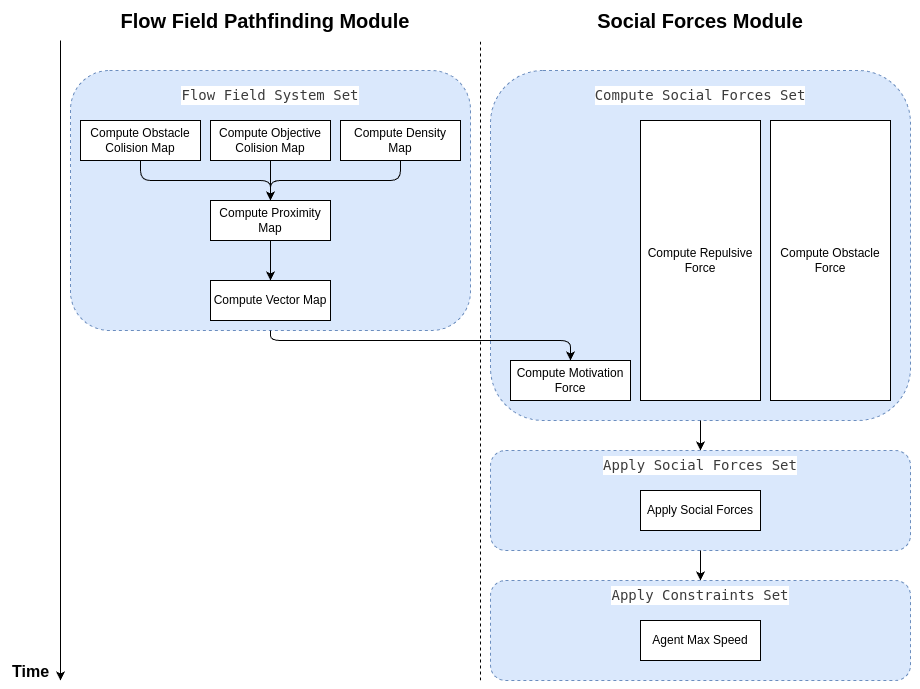
\includegraphics[width=\textwidth]{module_dependency.drawio.png}
  \caption[Example of how ECSMoS handles inter-module dependencies]{Example of how \gls{ecsmos} handles inter-module dependencies.}
  \label{fig:module_dependency}
\end{figure}

In the event that it becomes necessary to create a new module that has systems that must be executed after the first three systems of the Flow Field Pathfinding module, but that does not need to wait for the remaining systems, the current system sets are not sufficient. In this situation, the new module could create a new system set that exists on top of the current structure. This set can then only include the desired systems and be used for defining dependencies. 
\autoref{fig:module_dependency_example_module} shows an example of this. This new set can be anonymous and, as such, remain in use only inside the module or be given an identifier that would allow it to be used by other modules. Either way, it has no impact on the pre-existing system set or any of its relationships.

\begin{figure}[h]
  \centering
  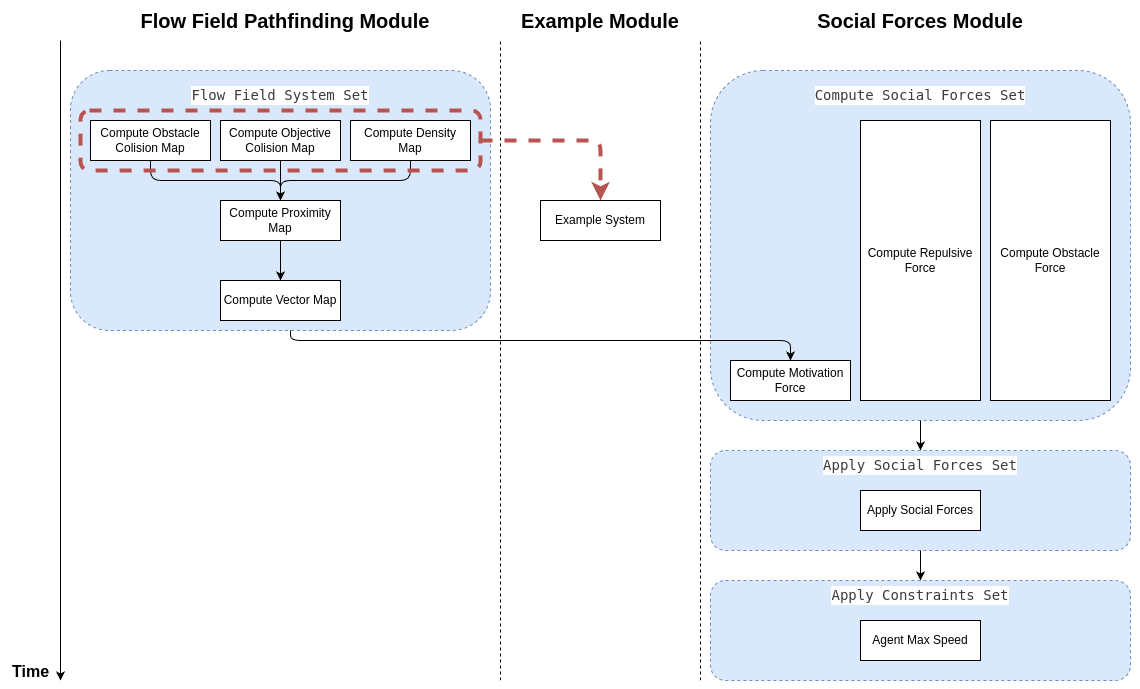
\includegraphics[width=\textwidth]{module_dependency_alt.drawio.png}
  \caption[Example of how ECSMoS handles the addition of systems with dependencies]{Example of how \gls{ecsmos} handles inter-module dependencies where there is no predefined system set grouping only the required systems. The thick dashed and rounded square represents the unnamed set created.}
  \label{fig:module_dependency_example_module}
\end{figure}

While generally a module is added as a whole. It is also possible to add only certain parts of it. For modules where there is a clear expectation that certain parts are only needed sometimes, it is possible to pass configuration variables to the module that enable or disable certain sections. If there was no expectation of this need during development, it is possible to bypass standard module initialization and add the required parts manually. While more time-consuming, this allows a large degree of control even over modules created by third parties. This is particularly useful when creating derivatives of pre-existing modules, as it allows the child module to only keep the parts of the parent that it desires while removing the others.

As a result of this approach, \gls{ecsmos} does not have a linear execution/relationship path between its modules like other simulators. Instead, it can be best imagined as a network, where each system is a node with its own relationships. Systems are generally more connected to other systems within the same module, but they often connect to other ones. While this increases the general flexibility of the simulator, it also comes with a drawback, as it allows for developers to unknowingly create circular dependency paths.

In its current state, \gls{ecsmos} has a simple \gls{ui} that is useful for debugging and visualizing the results during execution. The interface is built on top of Bevy's default rendering systems, which are relatively restrictive, but it is possible to add other \gls{ui} systems such as Bevy EGUI \cite{bevyegui}. This rendering functionality is not directly tied to the simulation state. There are systems that are executed at the end of each simulation loop that translate simulation data into values comprehensible by the \gls{ui} systems. As such, it is possible to add interface elements that are model-specific. 

Like Vadere, \gls{ecsmos} does not have a unified data collection or output mechanism. Both use data collectors, which only store certain fields, and post processors that output the collected data to one or multiple files. In both cases, a trajectory data collector is provided that is able to track the positions of pedestrians and export them in the \gls{csv} format or equivalent. However, more complex data collection may require additional systems to be created.

Finally, \gls{ecsmos} does not currently have a proper external file format for storing scenario definitions. Therefore, defining a scenario is currently done directly via code. Such a system is possible, but \gls{ecs} creates some additional complexities when it comes to this, most notably in the definition of system dependencies. There are many ways in which this could be accomplished, but it was considered outside the scope of the current work

\autoref{fig:simulator_ui} contains examples of the current UI of the simulator. \autoref{fig:general_ui} shows the general appearance of the simulator. The dots are agents, the circle to the left is their destination, and the rectangle to the right is where they are added to the simulation. On the top left, the counter shows how fast the simulation is going. Each frame is the equivalent of a simulation step. Figure \autoref{fig:vector_field} shows one of the many debug visualization modes. The one on display shows a field of vectors that point to the direction in which a pedestrian would go if it were in that location. Other debug modes include visualization of proximity to the target destination, collision zones, and statistical density of pedestrians. These modes are very useful for understanding the inner workings of the implemented model, but they impose a significant performance penalty.

\begin{figure}[h]
  \centering
  \begin{subfigure}{.5\textwidth}
    \centering
    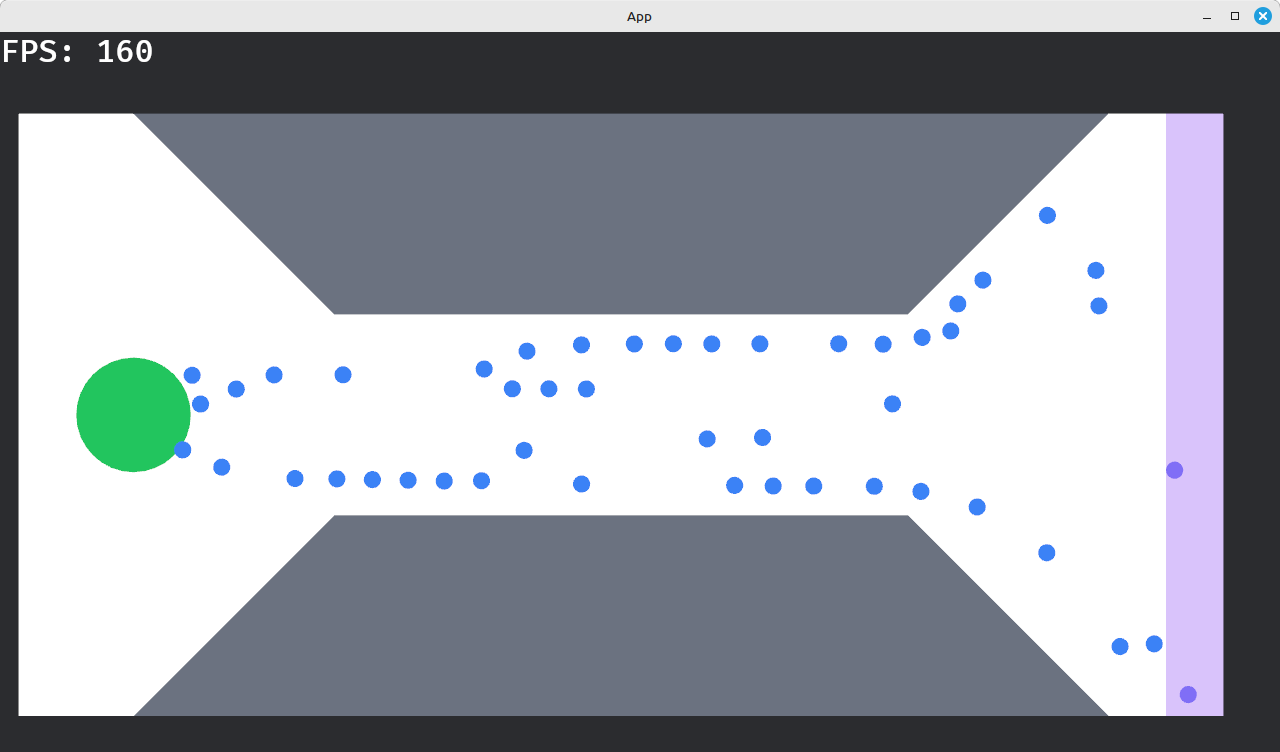
\includegraphics[width=.9\linewidth]{simulator_working.png}
    \caption[General \gls{ecsmos} \gls{ui}]{General \gls{ecsmos} \gls{ui}.}
    \label{fig:general_ui}
  \end{subfigure}%
  \begin{subfigure}{.5\textwidth}
    \centering
    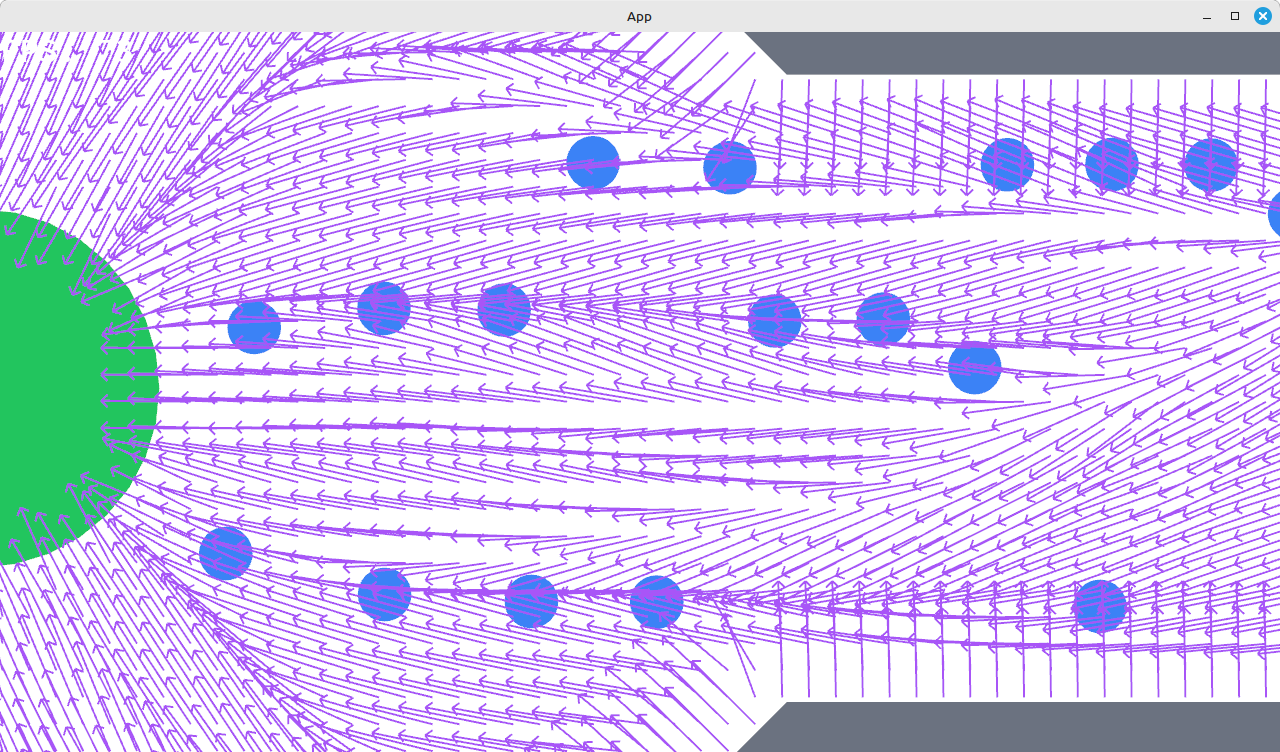
\includegraphics[width=.9\linewidth]{vector_field.png}
    \caption[Vector field \gls{ui}]{Vector field \gls{ui}.}
    \label{fig:vector_field}
  \end{subfigure}%
  \caption[\gls{ecsmos} interface]{\gls{ecsmos} interface.} 
  \label{fig:simulator_ui}
\end{figure}

\section{Evaluation} \label{sec:evaluation}

For the purposes of this work, two kinds of evaluations were defined for the simulator: qualitative and performance. The qualitative evaluation concerns itself with evaluating the usability, structure, reusability, and other similar aspects. In contrast, the performance evaluation consists of measuring its performance when compared to other simulators in similar test scenarios.  Of these two, the qualitative evaluation is arguably the most important. It focuses on comparing the capabilities of the simulators when it comes to the implementation of new models and adaptation of already existing ones. As such, it directly addresses the main objective of this project: flexibility. 

In addition to \gls{ecsmos}, two other simulators were selected for the comparison: Vadere and JuPedSim. These were chosen because they are the most robust ones still being updated. Out of the remaining simulators, MomenTUMv2 would also have been a suitable candidate due to the flexibility of its architecture. However, the fact that its continued development is uncertain and that it was left in a non-functioning state with no clear indication of which previous version could be considered usable meant that it was decided to remove it from the comparison. Conversely, jCrowdSimulator receives regular updates but was not considered for this comparison for lacking much of the basic infrastructure of a general simulator and due to its tightly coupled nature.

\subsection{Qualitative evaluation strategy} \label{sec:qualitative-evaluation}

For qualitative evaluation, a set of applications seen in the research was formalized and proposed as test use cases. \autoref{table:test-scenarios} contains a list of the use cases accompanied by their descriptions and main objectives. These were designed to test specific aspects of each simulator. However, they also had to be somewhat flexible to avoid hitting specific weak points of the simulators that could be easily avoided by slight shifts in the definition criteria. 

Firstly, Use Case 1 contains an example of this flexibility. The simulators being evaluated do not all use the same basic pathfinding system. Since the choice of pathfinding system is not an object of study in this dissertation, it was decided to define the use case in such a way as to allow for the use of any one of these. Similar accommodations have been made in the other use cases. 

Use Cases 1 to 3 test basic situations that are likely to arise during the development of most novel models. If a model is entirely novel, it would likely follow a path similar to Use Case 1. On the other hand, models that are largely based on an existing model but incorporate additional variables or factors would correspond to Use Case 2. Finally, Use Case 3 covers implementations that may not neatly fit into the previous categories.

Use Cases 4 and 6 target features that are less commonly used, but may present significant barriers during implementation. Some models explicitly consider how an agent makes decisions in a changing environment \cite{DEIULIIS2023104527}, while others include actions beyond movement, such as waiting in line or loitering \cite{KIM2013232, ALAM2022100527}. 

Moreover, a simulator's pathfinding algorithm may also have limitations or performance issues. These algorithms are used to compute the path pedestrians would attempt to take if the other agents around them were static and, for the \acrlong{sfm}, serve as the basis for the driving force. Vadere and \gls{ecsmos} use similar implementations that work well for the \gls{sfm} but generally perform worse for cellular automata models \cite{kleinmeierVadereOpenSourceSimulation2019}. As such, modifications may be necessary under certain circumstances, which is tested in Use Case 5.

After the use case definitions were stated, a study was conducted to implement them on each simulator. Implementations were then graded according to three metrics: implementability (ease of implementation), reusability, and complexity. These grades were given on a three-level scale: poor, fair, and good. Details of each level are described in \autoref{table:qualitative-evaluation-criteria}. In summary, a grade of "good" indicates that a simulator can easily handle the implementation of the use case, with minimal architectural challenges. A grade of "poor" implies significant challenges, potentially making the use case infeasible to implement. Finally, a grade of "fair" indicates manageable challenges that can be overcome with a reasonable level of effort.


\begin{center}
  \begin{table}[h!]
    \caption[List and description of use cases]{List and description of use cases.}
    \begin{tabularx}{\textwidth}{ | l | p{2.3cm}| X | p{5cm} | } 
      \hline
      \textnumero & Name & Description & Objective \\ 
      \hline
      1 & 
      New Model &  
      Add a new simple model that uses a basic pathfinding system already implemented on the simulator& 
      Test reusability of basic simulator infrastructure\\
      \hline
      2 & 
      Model \linebreak variation &  
      Create a variation of the \gls{sfm} available in the simulator with an additional attractive force that guides agents to areas where pedestrians would naturally concentrate, as defined in \cite{helbingSocialForceModel1995}& 
      Test reusability of existing model implementations when the variation is small\\
      \hline
      3 & 
      Hybrid model &  
      Create a model based on an already existing one that changes how it operates under some set of circumstances, similar to models that take panic into account, like those in \cite{Alrashed_Shamma_2020} & 
      Test general adaptability of already existing models to larger changes\\
      \hline
      4 & 
      Procedural \linebreak environment \linebreak changes &  
      Create a simulation environment that changes over time, adding new obstacles that change the pedestrian's paths as seen on \cite{DEIULIIS2023104527} & 
      Determine whether the simulator is able to handle updates to data that is not related to the pedestrians directly\\
      \hline
      5 & 
      New \linebreak pathfinding \linebreak algorithm &  
      Add a new algorithm for determining the shortest route between a pedestrian's current location and their destination& 
      Check the flexibility of current models to changes in base infrastructure, which may be necessary for performance or other limitations \cite{kleinmeierVadereOpenSourceSimulation2019}\\
      \hline
      6 & 
      Queuing \linebreak and \linebreak loitering&  
      Add procedures for pedestrians forming queues and for pedestrians staying still while waiting for something, but with some level of reactivity to the surrounding environment& 
      Queuing and loitering are behaviors that significantly change how a pedestrian moves and interacts with its environment. They also break many assumptions that are usually made by models, which often require continuous movement \cite{KIM2013232}\\
      \hline
    \end{tabularx}
    \label{table:test-scenarios}
  \end{table}
\end{center}

\begin{center}
  \begin{table}[h!]
    \caption[Description of evaluation criteria and their levels]{Description of evaluation criteria and their levels.}
    \begin{tabularx}{\textwidth}{ | p{2.9cm} | l | X | } 
      \hline
      Criteria & Grade & Description \\ 
      \hline
      Implementability & Good & 
      The simulator can easily accommodate the required additions. It has a clear place and method for receiving the new model, requiring minimal changes to existing code.
      \\ 
      \hline
      Implementability & Fair & 
      Implementation is feasible but requires moderate exploration of the code to identify where changes are needed or there are some tight coupling/rigid designs that slow down development.
      \\ 
      \hline
      Implementability & Poor & 
      Simulator lacks extension points for this use case, requires deep internal changes or requires modification to parts of its code that would be very difficult to decouple. Implementation is slow, messy or may not be feasible.
      \\
      \hline
      \hline
      Reusability & Good & 
      Existing code can easily be reused in this use case. The related models, utility methods, etc. are  generic, have good abstractions, and are composed of easily swappable units.
      \\ 
      \hline
      Reusability & Fair & 
      Some reuse is possible, but components are partially coupled to specific behaviors or use case. Reusing core infrastructure may impose minor restrictions or require small modifications. Model-specific logic may need to duplicate existing features if interfaces are too narrow or rigid.
      \\ 
      \hline
      Reusability & Poor & 
      Simulator components are hard-coded or specialized for specific agents or use cases. Implementing the scenario requires rewriting or duplicating most, if not all, of a model or internal system to operate. 
      \\ 
      \hline
      \hline
      Complexity & Good & 
      Implementing the use case is possible with minimal cognitive effort. The changes are well isolated, have logical continuity, touch as few other systems and the data/execution path they follow is direct and predictable.
      \\ 
      \hline
      Complexity & Fair & 
      Implementing the use case requires working with several components whose relationships aren't always intuitive. Changes may need to be performed in many regions of the code. Understanding the control flow is unintuitive or time-consuming, but possible.
      \\ 
      \hline
      Complexity & Poor & 
      Fully integrating the use case is very complicated. Control flow is chaotic, multiple tightly coupled parts have to be modified, or they may require a large redesign of the architecture of the simulator itself.
      \\ 
      \hline
    \end{tabularx}
    \label{table:qualitative-evaluation-criteria}
  \end{table}
\end{center}

\subsection{Performance evaluation strategy} \label{sec:performace-evaluation}

When it comes to scientific pedestrian simulation software, performance is often a secondary concern. For many applications, the total runtime of the simulator is acceptable as long as it does not impede or unreasonably slow down the research process. Given this context, the main objective of this evaluation is to measure the general effect of the change in architecture on the performance of the simulated models, rather than performing a comprehensive benchmark comparison.

Given no standard scenarios exist for performance comparison between pedestrian simulators, it was necessary to develop new ones. In line with the stated objective, minimizing the effects of other factors was paramount. Firstly, complex topologies disadvantage simulators such as JuPedSim, which determine base routes via polygon triangulation. The more polygons there are in a topology, the slower it is to compute the base paths of pedestrians. Conversely, large, empty spaces substantially increase the number of computations for simulators like Vadere and \gls{ecsmos}. These factors, independent of the underlying architecture, can cause non-linear performance drops that vary with both topology and pedestrian count. Therefore, scenarios were designed to minimize these effects.

Two scenarios were developed for this evaluation. \autoref{fig:performace_scenario_topologies} shows their physical topology. In these figures, black regions represent walls, green regions denote pedestrian spawners (locations where pedestrians are added at a specific frequency), and red regions represent destinations, where pedestrians are removed upon arrival. Each spawner is paired with a destination, indicated by letters. For example, pedestrians from spawner A aim for destination A.

\begin{figure}[h]
  \centering
  \begin{subfigure}{.33\textwidth}
    \centering
    \includesvg[width=.9\linewidth]{performance_scenario_1.svg}
    \caption[Scenario 1 -  Bottleneck]{Scenario 1 -  Bottleneck.}
    \label{fig:sfig1}
  \end{subfigure}%
  \begin{subfigure}{.67\textwidth}
    \centering
    \includesvg[width=.88\linewidth]{performance_scenario_2.svg}
    \caption[Scenario 2 - Corridor]{Scenario 2 - Corridor.}
    \label{fig:sfig1}
  \end{subfigure}%
  \caption[Performance scenario topologies]{Performance scenario topologies.}
  \label{fig:performace_scenario_topologies}
\end{figure}

Both developed scenarios feature simple topologies and relatively small surface areas. Nevertheless, they were designed based on real-world topologies commonly used during the development of novel pedestrian models. Scenario 1 reflects setups typically employed to evaluate the "Faster-Is-Slower Effect," in which increasing pedestrian speed can paradoxically reduce total throughput when a bottleneck is present. Scenario 2, in contrast, focuses on lane formation, a phenomenon in which pedestrians naturally organize into directional lanes when multiple streams moving in different directions intersect.

For these experiments, the frequency with which pedestrians are added to the simulation, denoted as $f_p$ and measured in $pedestrians/s$, was chosen as the main independent variable. This allows for the measurement of the performance of the simulators as the number of pedestrians, and therefore interactions, increases. For example, with $f_p = 0.5$, a pedestrian is added every other second, while $f_p = 8$ means that a pedestrian is added every 0.125 seconds. Agents are placed randomly inside their insertion regions and all have the objective of reaching their pre-assigned destination.

The dependent variable being measured during these tests was the total execution time. It was chosen because, for most scientific use cases, the total time it takes to execute a scenario is the most important property that is performance dependent. Other related metrics, such as mean time per simulation step, are not easily measurable in Jupedsim but can be derived from the mean total time. Each combination of scenario and $f_p$ was simulated 50 times, and the mean of the execution time was recorded.

All experiments use the Social Forces Model, with simulator constants standardized as shown in \autoref{table:sfm-constantns}. These include the calibration constants from \autoref{eq:pedestrian_repulsion}, \autoref{eq:pedestrian_obstacle}, and \autoref{eq:pedestrian_final_speed}. Since the algorithms used to compute the shortest path from a pedestrian to its destination, a key component of the motivation force, are substantially different and incompatible, their values were left at their default settings. The total amount of time simulated, denoted as $T_s$, was standardized to a value of 5 minutes, meaning that each run would simulate the equivalent of 5 minutes and then stop. This duration was chosen because it allows low and medium $f_p$ values to reach equilibrium, where the inflow and outflow of pedestrians are balanced, while preventing higher $f_p$ values from completely saturating the simulation area. Simulations were executed on standardized hardware, with key specifications listed in \autoref{table:pc-specs}.

\begin{table}[h]
  \caption[Controlled variables for the performance evaluation]{Controlled variables for the performance evaluation.}
  \begin{center}
    \begin{tabular}{ | l | c | c | } 
      \hline
      Parameter & Value & Unit\\ 
      \hline 
      $A_i$ & 2000 & $N$\\
      \hline
      $B_i$ & 0.08 & $m$\\
      \hline
      $k$ & 120000 & $\frac{kg}{s^2}$\\
      \hline
      $\kappa$ & 240000 & $\frac{kg}{m \cdot s}$\\
      \hline
      $r_i$ & 0.3 & $m$\\
      \hline
      $\tau$ & 0.5 & $s$\\
      \hline
      $v_i^0$ & 0.8 & $\frac{m}{s}$\\
      \hline
      $m$ & 80 & $kg$\\
      \hline
      $\Delta T$ & 0.1 & $s$\\
      \hline 
      $T_s$ & 5 & $min$\\
      \hline 
    \end{tabular}
    \label{table:sfm-constantns}
  \end{center}
\end{table}

\begin{table}[h]
  \begin{center}
    \caption[Simulation hardware and software]{Simulation hardware and software.}
    \begin{tabular}{ | l | c | } 
      \hline
      Property & Value \\ 
      \hline 
      Operating System & Linux Mint 22.1 Cinnamon \\
      \hline
      Linux Kernel & 6.8.0-71-generic \\
      \hline
      CPU & AMD Ryzen 5 5560U \\
      \hline
      Graphics Card & AMD Radeon Vega Mobile Series \\
      \hline
      RAM & 12 GB \\
      \hline
    \end{tabular}
    \label{table:pc-specs}
  \end{center}
\end{table}


\subsection{Qualitative evaluation results}

Following the directives outlined in \autoref{sec:qualitative-evaluation}, each use case was implemented in sequence. Whenever examples, extension points, or documentation provided by the developers suggested a recommended implementation approach, these guidelines were followed. In the absence of such explicit directions, multiple alternative solutions were explored to determine the most suitable one according to the defined evaluation criteria. The results of this process, along with additional commentary, are presented below.

\begin{center}
  \begin{table}
    \caption[Summary of qualitative results]{Summary of qualitative results.}
    \begin{tabularx}{\textwidth}{ | p{3.7cm} | X | X | X | X | X | X | X | X | X | } 
      \hline
      \backslashbox{Use Case}{Simulator} & 
      \multicolumn{3}{|c|}{\gls{ecsmos}} & 
      \multicolumn{3}{|c|}{Vadere} & 
      \multicolumn{3}{|c|}{JuPedSim} 
      \\
      \hline
      &
      \rotatebox[origin=c]{90}{\hphantom{O}Implementability\hphantom{O}} &
      \rotatebox[origin=c]{90}{Reusability} &
      \rotatebox[origin=c]{90}{Complexity} &

      \rotatebox[origin=c]{90}{Implementability} &
      \rotatebox[origin=c]{90}{Reusability} &
      \rotatebox[origin=c]{90}{Complexity} &

      \rotatebox[origin=c]{90}{Implementability} &
      \rotatebox[origin=c]{90}{Reusability} &
      \rotatebox[origin=c]{90}{Complexity} 
      \\ 
      \hline
      (1) New Model & 
      Good & Good & Fair & 
      Good & Good & Good & 
      Fair & Fair & Fair\\
      \hline
      (2) Model variation & 
      Good & Good & Fair & 
      Good & Fair & Good & 
      Fair & Fair & Fair\\
      \hline
      (3) Hybrid model & 
      Good & Good & Fair & 
      Good & Fair & Good & 
      Fair & Fair & Fair \\
      \hline
      (4) Procedural environment changes &
      Good & Good & Fair &
      Fair & Fair & Poor &
      Poor & Poor & Poor \\
      \hline
      (5) New pathfinding algorithm &
      Good & Fair & Fair &
      Poor & Fair & Poor &
      Fair & Fair & Fair \\
      \hline
      (6) Queuing and loitering&
      Good & Good & Fair &
      Good & Poor & Good &
      Good & Good & Good \\
      \hline
    \end{tabularx}
    \label{table:qualitative-summary}
  \end{table}
\end{center}

Each simulator had very similar results in Use Cases 1, 2, and 3. These use cases are not complicated and serve primarily as a baseline for comparison with the more complex ones. Nonetheless, they already reveal several trends that persist throughout most of the remaining use cases. Firstly, even in these basic use cases, \gls{ecsmos} exhibits a higher level of complexity than desired, largely due to the open-ended nature of its architecture. Since new systems can be inserted at any point within the simulation schedule, understanding the overall control flow often becomes challenging in practice. On the other hand, implementing model variations and hybrid models is simple: such extensions can be added on top of existing models by adding a few systems that work together with the pre-existing ones.

Secondly, JuPedSim generally performs worse than the others being studied under these criteria. Such a pattern stems from its highly coupled internal structure. Even in basic use cases, JuPedSim necessitates numerous modifications all around the codebase in the form of string comparisons and other conditional mechanisms that define how execution will go depending on each model. This issue is most notable in the interface between Python and C++ code, where there are large sections of model-specific code that are executed depending on a sequence of chained conditions.

Finally, Vadere receives a lower reusability scores starting on Use Case 2 due to the fact that its existing model implementations have a somewhat limited level of extensibility. With better choices when it comes to how the code is divided or how classes and interfaces are structured, it could cut down on the amount of code duplication significantly.

Use Case 4 introduces additional challenges when it comes to flexibility. Both Vadere and JuPedSim encounter difficulties on this front, as they assume static environments. This is a reasonable expectation for some simpler situations, but that is not a universal property. Within Vadere, it is still possible to accommodate these with some work, but it will require reengineering some portions of the simulator itself. In contrast, implementing these features in JuPedSim is practically unfeasible, as it would require reengineering most of the simulator. In comparison, \gls{ecsmos} handles such things much better. Bevy ECS provides methods for detecting this kind of changes and, in many situations, these can be added with little to no modification to the code of the systems themselves. In the situation where changes to the systems are necessary, those are limited and much more predictable. 

Use Case 5 causes a reversal in the grades between Vadere and JuPedSim. Vadere's pathfinding algorithm, known as floor fields, is much more  integrated with the simulator's architecture and existing models, whereas JuPedSim relies on triangulation to determine the best possible path for each pedestrian. Although floor fields could theoretically be replaced with an alternative mechanism, it would require extensive modifications to both the simulator code and all existing model implementations, making it impractical. In contrast, \gls{ecsmos} supports such changes seamlessly. While code reuse between the current pathfinding system and a new one may be limited, the architecture itself does not introduce additional obstacles, and the modifications required to enable existing models to utilize the new system are minimal and localized.

Finally, in Use Case 6, JuPedSim performs very well. Its architecture is specifically designed to accommodate this type of behavior, making it both well-integrated and highly flexible. Although \gls{ecsmos} was not explicitly designed for this use case, similar functionality can be achieved using the same approach as in Use Case 3 for hybrid models, where queuing and loitering are implemented as extensions on top of the already available model. In theory, Vadere could adopt a similar approach to \gls{ecsmos}, but in practice, this would require rewriting the entire model to account for these behaviors due to inherent limitations in its extensibility. Therefore, Vadere receives a lower score in the reusability criteria.


As the results in \autoref{table:qualitative-summary} show, Vadere and \gls{ecsmos} are the best for basic use cases, with Vadere holding a slight advantage. Each one has its strong and weak points, but both are generally suitable for implementing a novel pedestrian model that does not involve complex dynamics, such as environmental changes. However, when use cases require more sophisticated modifications, \gls{ecsmos} demonstrates a clear advantage due to its superior flexibility. In comparison, JuPedSim generally yields worse results across the use cases, with its only standout result in Use Case


\subsection{Performance evaluation results}

Similarly to the qualitative results, the performance results were very close for the less demanding scenarios, while diverging significantly on later ones. \autoref{fig:performace-results} shows the full results in detail. In the graph, scenarios are identifiable by the shape of the markers, while each simulator is represented by a distinct color. The shaded areas surrounding each trend line indicate the standard deviation of the measurements, reflecting the variability of the results.

As can be observed, the performance across simulators and scenarios is very similar for lower values of $f_p$. With such low pedestrian densities, the base costs of loading data into memory, pre-processing, and post-processing dominate the overall runtime. Some variation remains, most notably from Vadere, which is written in Java and therefore exhibits comparatively slower performance, as Java is not fully compiled but instead partially compiled into an intermediate language that must be interpreted at runtime. JuPedSim, which uses Python, an interpreted language, has higher performance because the core computations are implemented in C++. Python is mostly used as a wrapper for a convenient interface that delegates execution directly to the C++ layer.

Starting at $f_p = 3$, no data is available for JuPedSim in Scenario 2, and by $f_p = 6$, the same limitation occurs for Scenario 1. This issue comes from a limitation in JuPedSim. As pedestrian densities increase inside the simulation, it is possible for the repulsive interaction between pedestrians to become too strong in certain circumstances. These strong forces can cause an individual to move at such a high speed that its position in the next simulation loop goes over the barriers that limit the simulation area, causing the agent to appear outside the simulation area. This behavior is a common issue in both simulators and games, and stems from a simplification in the collision detection algorithm. Rather than verifying whether a pedestrian's path would intersect a wall, the code simply checks for the presence of a wall at the location the agent will be in the next simulation step. At low speeds this approach is sufficient, but it has limited applicability at higher speeds.

Such high speeds are not usually possible for pedestrians in the real world, but similar situations can arise in many models, including the Social Forces Model. A common location for this to happen is near regions where pedestrians are added. In these locations, a new pedestrian may be added much closer to others than would normally be possible, creating unusually large repulsive forces. Both Vadere and \gls{ecsmos} mitigate this issue by enforcing a configurable maximum speed, set well below the threshold that could lead to such problems. Since such speeds are physically impossible in real-world scenarios, the maximum speed constraint helps to ensure the model behaves more realistically. However, JuPedSim lacks this safeguard and any means to configure it. As a result, even moderate pedestrian densities can cause failures in certain situations. While this does not occur in every simulation run, it becomes frequent enough at $f_p = 3$ and $f_p = 6$ to make it infeasible to obtain representative results.

Vadere and \gls{ecsmos} exhibit an overall quadratic growth in simulation duration as $f_p$ increases. While various optimization strategies exist, this behavior is an inherent consequence of the Social Forces Model. Each pedestrian both applies forces to others and experiences reciprocal forces from them. These must be computed for every pair of agents, leading to a computation cost that grows quadratically with the number of agents in the simulation. However, at higher frequencies , a large difference in performance emerges between the two. Still, it is challenging to quantify how much of this difference is attributable to architectural design versus the underlying programming language.

\begin{figure}
  \centering
  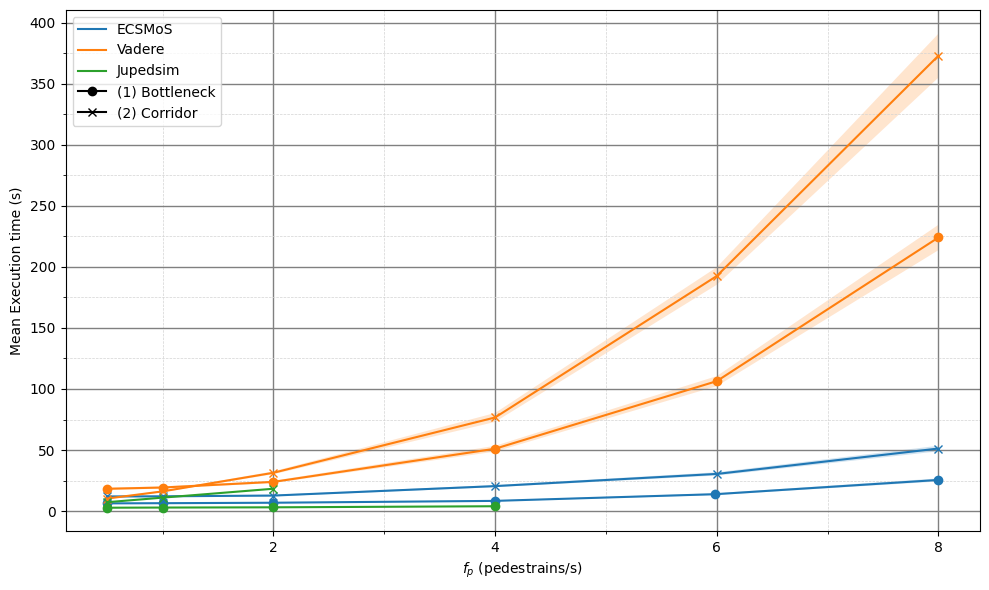
\includegraphics[width=\textwidth]{performace_result.png}
  \caption[Summary of performance results]{Summary of performance results.}
  \label{fig:performace-results}
\end{figure}

Comparing \gls{ecsmos} to JuPedSim is simpler when it comes to the performance of their respective programming languages, as C++ and Rust have very similar performance profiles \cite{electronics12010143}. In the proposed scenarios, both simulators have nearly identical performance at lower frequencies. This suggests that their architectures may be roughly equivalent in terms of performance. However, due to the lack of data for the later runs for JuPedSim, it is not possible to make reliable conclusions about their relative performance in more demanding scenarios.




\section{Conclusion} \label{sec:conclusion}

This research aimed to determine the benefits and drawbacks of introducing the \gls{ecs} architecture into the realm of scientific pedestrian simulations with a focus on flexibility. As part of this, the area of pedestrian simulations was studied, including currently available pedestrian models and a survey of pedestrian simulators. With this context established, the characteristics of the \gls{ecs} architecture were laid out in comparison to the ones used by current simulators. Finally, a novel simulation framework, \gls{ecsmos}, was proposed, developed and compared against some of the most popular pedestrian simulators, Vadere and JuPedSim.

The results of the qualitative analysis show that \gls{ecsmos} is more flexible when compared to the other subjects of study overall, with special highlights in situations that require procedural environment changes, where both of the other simulators face significant challenges. However, this comes at the expense of complexity. In fact, \gls{ecsmos} is generally more complex than the alternatives in simpler scenarios. However, this drawback becomes less relevant when finer control or flexibility is required. In terms of performance, \gls{ecsmos} is just as or more performant than the alternatives in all studied scenarios. Still, these results are not fully comparable, as there are other significant factors that may affect performance that cannot be isolated.

Based on these results, it is possible to conclude that \gls{ecs} is a viable alternative to currently accepted programming paradigms used in the simulation of pedestrians. Its benefits come in the form of flexibility and control, but they come with drawbacks in terms of required learning for unfamiliar researchers and a generally complex execution flow and debugging procedures. Therefore, it is best used for implementing models that require features that are not currently standard or break the general assumptions when it comes to pedestrian model structure.

Future works in exploring the limits of the \gls{ecs} architecture should focus on expanding the current simulation core with features necessary for a fully fledged simulator. These may include a better UI, mechanisms for defining scenarios via external files, better data gathering, supporting other export formats, and many others. Additionally, it may be possible to use some of the strategies and concepts of \gls{ecs} on other simulators. This path of research may allow researchers to have the benefits of \gls{ecs} without needing to go through the sharp learning curve associated with \gls{ecs} and Rust.

\printbibliography

\end{document}